\chapter[Introdução]{Introdução}

De acordo com o SNT (Sistema Nacional de Transplante), o Brasil possui um dos maiores programas públicos de transplante de órgãos e tecidos do mundo. Apesar deste importante avanço, a estrutura de processos administrativos e operacionais ainda é deficiente e causa grande impacto na viabilidade e ocorrência do transplante. Em 2005 existiam cerca de 60 mil brasileiros na fila de espera por um transplante de órgãos, sendo que destes apenas 20\% seriam atendidos, sendo o maior fator contribuinte para a não realização do procedimento, a estrutura deficiente de captação e distribuição de órgãos (Bergamo, 2005), e não a falta de doadores.
Desta forma, sabe-se que a melhoria no processo logístico causará impactos positivos no cenário brasileiro de transplante de órgãos, beneficiando os milhares de brasileiros que se encontram na fila de espera por um órgão. 

\section{Contexto}

A história da transplantação de órgãos é recente, iniciada na década de 1960 no Brasil e marcada por grandes avanços no enfoque da medicina e da tecnologia desde então, o que atualmente permite melhores perspectivas sobre saúde e longevidade. A regulamentação dos transplantes de órgãos aconteceu no Brasil no ano de 1997 pela Lei nº 9.434, e adicionalmente a ela o Decreto nº 2.268/1997 criou o Sistema Nacional de Transplantes responsável pela captação e distribuição de órgãos e tecidos. O Registro Brasileiro de Transplantes (RBT) mostra o crescimento dos casos de transplantação no ano de 2016, com destaque para o transplante hepático, com aumento nacional de 3,9\%, e para o transplante de pâncreas, com aumento nacional de 11,7\%, se comparados ao ano de 2015.

Para melhor compreensão deste estudo, define-se transplante como uma substituição cirúrgica de um órgão ou tecido afetado por lesão progressiva e irreversível por um outro sadio, de doador falecido ou vivo \cite{neto}. O êxito nas atividades de transplantação está atrelado não só ao procedimento cirúrgico, mas anteriormente, e também, ao bom manejo do órgão que envolve a excelência no procedimento de acondicionamento para transporte. Uma falha na logística de transporte e/ou em seu armazenamento podem apresentar riscos ao futuro transplantado, além da falência do órgão.

Neste contexto, aprimorar os recursos tecnológicos, a fim de tornar as condições de armazenamento tão excelentes quanto o necessário para garantir o funcionamento e integridade ao recurso vindo de um doador é fundamental. Os riscos que podem vir a tornar inviável a transplantação devem ser drasticamente minimizados, pois os dados mostram que a proporção é de um doador para cada 8 potenciais doadores de órgão (ABTO, 2009), ou seja, os recursos têm de ser manejados da melhor forma possível para eliminar as possibilidades de inutilização do órgão.
	
Para o desenvolvimento de um equipamento de acondicionamento de órgãos adequado, torna-se imprescindível o conhecimento de todas as normas e requisitos que garantem as melhores condições de armazenamento durante o transporte. A Associação Brasileira de Transporte de Órgãos traz informações sobre os máximos tempos de permanência extracorpórea dos recursos, como mostra a tab. \ref{preservacao_extracorporea}:

\begin{table}[h!]
\centering
\begin{tabular}{|l|l|l|}
\hline
\textbf{Órgão/Tecido} & \textbf{\begin{tabular}[c]{@{}l@{}}Tempo máximo \\ para retirada\end{tabular}} & \textbf{\begin{tabular}[c]{@{}l@{}}Tempo máximo de \\ preservação extracorpórea\end{tabular}} \\ \hline
Córneas               & 6 horas após PC*                                                               & 7 dias                                                                                        \\ \hline
Coração               & Antes da PC*                                                                   & 4 a 6 horas                                                                                   \\ \hline
Pulmão                & Antes da PC*                                                                   & 4 a 6 horas                                                                                   \\ \hline
Rins                  & Até 30 min. pós PC*                                                            & Até 48 horas                                                                                  \\ \hline
Fígado                & Antes da PC*                                                                   & 12 a 24 horas                                                                                 \\ \hline
Pâncreas              & Antes da PC*                                                                   & 12 a 24 horas                                                                                 \\ \hline
Ossos                 & 6 horas pós PC*                                                                & Até 5 anos                                                                                    \\ \hline
\end{tabular}
\caption{Tempo máximo de preservação extracorpórea (ABTO, 2011)}
\label{preservacao_extracorporea}
\end{table}

A Agência Nacional de Vigilância Sanitária (ANVISA) estabeleceu, pela Resolução RDC nº 66/2009, as condições sanitárias de transporte de órgãos humanos, e regulamenta o funcionamento da acomodação e  transporte destes recursos. Os principais requisitos desta norma quanto ao sistema de armazenagem são:

\begin{citacao}


Art. 31. A embalagem primária deve conter o órgão e a solução de preservação, e ter capacidade proporcional ao volume do órgão a ser embalado.

 Art. 32. A embalagem primária deve ser acondicionada em duas embalagens secundárias.
 
Art. 36. As embalagens secundárias devem ser acondicionadas na embalagem terciária.

 Art. 37. A embalagem terciária será constituída de caixa isotérmica confeccionada de material rígido, resistente e impermeável, deverá promover isolamento térmico, ser revestida internamente com material liso, durável, impermeável, lavável e resistente a soluções desinfetantes e conter um dispositivo de segurança que impeça sua abertura acidental. 
 
Art. 38. A embalagem terciária deve ser preenchida com gelo (ponto de fusão a 0\degree C) em quantidade suficiente para envolver a embalagem secundária e garantir a manutenção da temperatura pelo tempo necessário do processo de transporte. 

Art. 39. O gelo com ponto de fusão a 0\degree C utilizado não deve entrar em contato direto com os órgãos. 

Art. 40. É vedado o emprego de solução salina congelada como material refrigerante no acondicionamento, para prevenir congelamento do órgão.  

\end{citacao}

Ademais, cada órgão possui suas próprias especificações que devem ser respeitadas. O armazenamento do fígado e pâncreas, por exemplo, são realizados sob as mesmas condições, entretanto, separadamente. O órgão é colocado separadamente no interior de um saco plástico estéril contendo 1 litro de solução Viaspan (solução para conservação de órgãos) a 4\degree C e lacrado com fita cardíaca. Após, o saco é posto no interior de outro saco plástico estéril com gelo moído e novamente lacrado com fita cardíaca. Identifica-se com um cartão que contém o horário de clampeamento, e este conjunto deve permanecer em geladeira térmica, coberto com gelo não estéril até a utilização dos enxertos (NETO; AFONSO; THOMÉ, 2010).

Alternativamente ao emprego de um sistema de refrigeração manual, este projeto visa a concretização de uma caixa, em concordância com a embalagem terciária do artigo 37 da Resolução RDC nº 66/2009, com um sistema de resfriamento que não se utiliza de gelo não estéril e com a possibilidade de controle e verificações de suas condições de atuação, visando propiciar melhores condições de armazenamento e transporte de órgãos.


\section{Justificativa}

Atualmente no transporte de órgãos, utilizam-se caixas térmicas, onde o órgão é depositado em soro e coberto por embalagens com gelo. Podem acontecer casos de perda e deterioração prematura do órgão, devido à queima do tecido pelo contato não homogêneo com as embalagens de gelo. De acordo com o Dr. Fernando A. G. Guimarães,em sua tese de mestrado “Câmara Hiperbárica refrigerada para a preservação de órgãos e tecidos”, é notável uma melhor preservação do órgão em sistemas pressurizados com oxigênio puro e temperatura controlada.

Além dos processos de acondicionamento, armazenagem e transporte, é necessário levar em consideração o tempo de isquemia de cada órgão, que consiste no intervalo entre a retirada e acondicionamento em solução própria e a inserção do órgão no corpo do receptor,  e as distâncias entre os doadores e os receptores. Este tempo será monitorado pelo sistema de acompanhamento de órgão, para que não haja atraso e a consequente deterioração do tecido antes da chegada ao destino.


\begin{table}[h!]
\centering
\begin{tabular}{|l|l|}
\hline
\textbf{Órgão} & \textbf{Tempo de Isquemia Fria} \\ \hline
Coração        & 4 horas                         \\ \hline
Pulmão         & 4-6 horas                       \\ \hline
Fígado         & 12 horas                        \\ \hline
Rim            & Até 24 horas                    \\ \hline
Pâncreas       & Até 20 horas                    \\ \hline
\end{tabular}
\caption{Tempo de isquemia por órgão(ABTO, 2009)}\label{isquemia_orgaos}
\end{table}

\section{Escopo do projeto}
 \subsection{Premissas}
  \begin{itemize}
    \item Os órgão devem ser condicionados em uma câmara selada hermeticamente.
    \item A câmara deverá ser resfriada e manter-se entre 2 e 4 graus Celsius.
    \item O transportador só poderá ser aberto no seu destino.
    \item Haverá comunicação com a internet para que o hospital que receberá o órgão possa acompanhar o andamento da entrega.
  \end{itemize}

  \subsection{Restrições}
  \begin{itemize}
    \item O órgão não poderá ser necrosado por falta de refrigeração nem queimado por excesso dela.
    \item A caixa transportadora deverá ser dimensionada de forma que duas pessoas adultas possam carregá-la.
    \item O sistema de fechamento não será aberto até a chegada no destino do órgão.
    \item O sistema de transporte deverá estar de acordo com a legislação vigente, se for aplicável.

  \end{itemize}

\section{Detalhamento do escopo}
  \subsection{Projeto}
  O grupo do Transportador de Órgãos da disciplina de Projeto Integrador 2, visa suprir a necessidade de um controle maior na importantíssima atividade de transportar órgãos humanos para transplante, buscando o maior controle das características do transporte para que a chance real do órgão chegar a tempo e de forma útil para quem irá recebê-lo. O órgão será acondicionado dentro de três camadas de materiais que tratarão de isolar termicamente e hermeticamente de forma que o órgão chegue saudável a seu destino.

  O público alvo do projeto são as equipes de transplante que agem para salvar vidas levando essa importante carga por todo o país, seja de avião, helicóptero, ambulância ou qualquer outro meio de locomoção. O objetivo é facilitar o controle e a entrega dos órgãos para seus recebedores.

  \subsection{Produto}
  O sistema de automatização do recipiente do transporte facilitará o controle de temperatura, que ocorrerá automaticamente, terá sistema energético próprio aumentando sua autonomia e se conectará com a internet para que o seu destino saiba onde o órgão está e quais suas características em tempo real. Se o lugar for remoto e não houver conexão, assim que a conexão for estabelecida os dados serão atualizados.

  O sistema funcionará da seguinte forma: O órgão será introduzido dentro da câmara de resfriamento que por sua vez será selada hermeticamente. O resfriamento da câmara já deve ter ocorrido para que o órgão seja resfriado o mais rápido possível. O segundo invólucro que terá o isolamento térmico será fechado e trancado para que só possa ser aberto em seu destino. No trajeto o órgão será observado por sensores de temperatura e pressão enquanto a localização do sistema e esses dados são transmitidos pela internet para um servidor que pode ser acessado via um aplicativo na internet. Chegado em seu destino o órgão poderá ser retirado para o transplante.

  O sistema completo poderá ficar pesado para uma pessoa levar, por isso a estrutura poderá ter rodas que facilitam sua locomoção, mas será dimensionado, o projeto, de forma que duas pessoas possam levantá-lo sem problemas para colocá-lo em qualquer veículo.

  Para que o projeto seja considerado um sucesso este deverá atender aos seguintes quesitos: manter a temperatura o isolamento e a pressão do órgão até sua chegada no destino, não podendo ser aberto até então e que passe todas essas informações para que os interessados saibam as características do órgão e onde está o transporte.


\section{Objetivos}

\subsection{Objetivo Geral}

Tendo em vista os obstáculos e desafios enfrentados no transporte de órgãos hodiernamente, sem deixar de levar em consideração a sua relevância social, o presente trabalho propõe a concepção de um sistema automatizado de transporte de órgãos, levando em conta as condições específicas de contorno necessárias para a preservação de cada órgão durante o tempo de translado. O grupo, então, orientará seus esforços no sentido de conceber um sistema que preserva órgãos específicos, contando com o trabalho harmônico e sinérgico de cada uma das áreas do conhecimento de seus membros.

\subsection{Objetivos Específicos}

Levando em consideração os objetivos gerais acima propostos, e utilizando-os como diretriz, citam-se os objetivos específicos logo abaixo:

\begin{itemize}
	\item Projetar e construir a estrutura da câmara onde o órgão será acondicionado, seguindo todas as normas de assepsia e acondicionamento propostas pela ANVISA;
    \item Projetar e implementar o sistema de controle e coleta de dados em tempo real, utilizando o microcontrolador MSP430g2553;
	\item Projetar e implementar o sistema que analisará, processará e enviará os dados coletados para uma plataforma WEB através de uma plataforma GPRS, com auxílio da RaspBerry PI;
	\item Projetar o sistema que fará a tomada de decisões, que se dará através da comunicação entre o RaspBerry PI e MSP430g2553; 

\item Projeto e implementação da plataforma WEB;
	\item Análise de transferência de calor da câmara, de forma que tal transferência ocorra da forma correta, sem danificar o tecido do órgão. 
\end{itemize}

\section{Metodologia de gerenciamento}

A metodologia ágil, mais especificamente o SCRUM, tem como princípio agregar valor ao cliente de maneira mais rápida possível a partir de uma gerência eficiente das pessoas envolvidas e suas respectivas funções. O PMBOK é referência em gerenciamento de projetos por conter artefatos e boas práticas que ajudam a desenvolver um projeto de maneira eficaz. Na realização do projeto do transporte de órgãos será utilizada uma combinação do SCRUM e do PMBOK.

O SCRUM será utilizado para organizar o esforço de trabalho dos participantes em sprints semanais, que terão planejamento e retrospectiva, além disso teremos reuniões diárias através da plataforma online SLACK tendo visibilidade do trabalho executado por cada membro e frente de trabalho.

Do PMBOK utilizaremos alguns artefatos para documentação do projeto como:

\begin{itemize}
	\item Plano de gerenciamento de comunicação
	\item Plano de gerenciamento de requisitos
    \item Plano de gerenciamento de riscos
    \item Plano de gerenciamento de custos
\end{itemize}

\subsection{Plano de gerenciamento de comunicação}

O plano de gerenciamento das comunicações tem a finalidade de abordar os meios de comunicação utilizados no desenvolvimento do transportador de órgãos desenvolvido como projeto da disciplina de Projeto Integrador de Engenharia 2. A comunicação se faz importante para o sucesso ou falha de projeto e interfere diretamente no conhecimento compartilhado entre a equipe.

Nesta subseção será descrito aspectos relevantes para o gerenciamento de comunicação como a frequência de encontros e as ferramentas utilizadas para obter uma forte integração entre a equipe.

\subsubsection{Agenda semanal/Reuniões}

A equipe trabalha no contexto de reunião física durante as aulas e no contexto de comunicação externa fora das aulas, portanto as reuniões são estruturadas de forma a extrair a maior produtividade dos integrantes durante as aulas.
As reuniões permitem trocas de informações entre a equipe, proporcionando melhorias no desenvolvimento geral do time.

\begin{table}[H]
\centering

\begin{tabular}{|l|l|l|l|l|}
\hline
\textbf{Motivo}                                                            & \textbf{Participantes}                                         & \textbf{Método}                                                      & \textbf{Frequência}                                                              & \textbf{Dia} \\ \hline
Reunião fixa                                                               & \begin{tabular}[c]{@{}l@{}}Todos \\ os membros\end{tabular}    & Presencial                                                           & \begin{tabular}[c]{@{}l@{}}Uma vez \\ por semana. \\ 16:00 às 18:00\end{tabular} & Quarta-feira \\ \hline
Reunião fixa                                                               & \begin{tabular}[c]{@{}l@{}}Todos\\ os membros\end{tabular}     & Presencial                                                           & \begin{tabular}[c]{@{}l@{}}Uma vez \\ por semana. \\ 14:00 às 18:00\end{tabular} & Sexta-feira  \\ \hline
\begin{tabular}[c]{@{}l@{}}Reuniões de \\ frentes de trabalho\end{tabular} & \begin{tabular}[c]{@{}l@{}}Frentes \\ de trabalho\end{tabular} & \begin{tabular}[c]{@{}l@{}}Reunião \\ digial \\ (hangout)\end{tabular}  & \begin{tabular}[c]{@{}l@{}}Quando forem \\ necessárias\end{tabular}              & -            \\ \hline
Reunião de gerência                                                        & \begin{tabular}[c]{@{}l@{}}Equipes \\ de gerência\end{tabular} & \begin{tabular}[c]{@{}l@{}}Reunião \\ digital \\ (hnagout)\end{tabular} & 2 vezes por semana                                                               & -            \\ \hline
\end{tabular}
\caption{Plano de comunicações}
\label{plano_comunicacao}
\end{table}

\subsubsection{Tecnologia de comunicação}

\begin{table}[H]
\centering
\begin{tabular}{|l|l|l|l|}
\hline
\textbf{Tecnologia} & \textbf{\begin{tabular}[c]{@{}l@{}}Urgência \\ das informações\end{tabular}} & \textbf{Objetivo}                                                                                           & \textbf{\begin{tabular}[c]{@{}l@{}}Métodos \\ de comunicação\end{tabular}} \\ \hline
Whatsapp            & Alta                                                                         & \begin{tabular}[c]{@{}l@{}}Comunicação rápida\\  e informal\end{tabular}                                    & Comunicação interativa                                                     \\ \hline
Slack               & Alta                                                                         & \begin{tabular}[c]{@{}l@{}}Acompanhamento \\ de desenvolvimento\end{tabular}                                & Comunicação interativa                                                     \\ \hline
Google Drive        & Baixa                                                                        & \begin{tabular}[c]{@{}l@{}}Armazenamento, \\ compartilhamento\\  e produção de documentos\end{tabular}      & Comunicação passiva                                                        \\ \hline
Hangouts            & Média                                                                        & Reuniões online                                                                                             & Comunicação interativa                                                     \\ \hline
Git                 & Baixa                                                                        & \begin{tabular}[c]{@{}l@{}}Versionar as informações\\ dos relatórios do grupo\end{tabular}                  & Comunicação passiva                                                        \\ \hline
Trello              & Alta                                                                         & \begin{tabular}[c]{@{}l@{}}Acompanhamento \\ do processo \\ de desenvolvimento \\ e atividades\end{tabular} & Comunicação passiva                                                        \\ \hline
\end{tabular}
\caption{Tecnologias de comunicação}
\label{tec_comunicacao}
\end{table}

\subsubsection{Monitoramento e Controle}

Os integrantes devem ser pontuais e comunicativos nas reuniões, fazendo o uso das ferramentas e meios de comunicação definidos a priori. Será feito um Registro de Presença para monitorar a presença dos integrantes e está diretamente relacionada à participação dos membros no projeto. Para controle de trabalho e comunicação será utilizada como ferramenta principal o Trello, onde todo o trabalho terá responsável e tempo para ser terminado.

\subsection{Plano de gerenciamento de riscos}
Os riscos do projeto foram avaliados e estão descritos na Tabela \ref{tab:riscos}. Foram analisados a probabilidade de acontecerem os eventos e quão impactante eles serão, caso ocorram.

\footnotesize  % Switch from 12pt to 11pt; otherwise, table won't fit
\setlength{\LTleft}{-35pt}            % default: \fill
\setlength{\LTright}{\fill}           % default: \fill
\begin{longtable}{|m{2.8cm}|m{4cm}|m{2.5cm}|m{2.2cm}|m{4cm}|}
\caption{Riscos para todos os subsistemas}
\label{tab:riscos} 
\endfirsthead
\endhead
\hline
\textbf{Risco}            & \textbf{Consequência}               & \textbf{Probabilidade}                         & \textbf{Impacto}                 & \textbf{Ação/estratégia}              \\ \hline
\multicolumn{5}{|c|}{\textbf{Geral}}\tabularnewline \hline

Atraso no cronograma & Sobrecarregamento em certos períodos do projeto e/ou  atraso na entrega do produto final. & Provável. & Razoavelmente impactante. & Ajuste ou  remodelamento  de atividades a  serem  desenvolvidas. \\ \hline

Erro de planejamento                                              & Replanejamento do projeto e/ou atraso na entrega do produto final.                             & Razoavelmente provável. & Muito impactante.         & Replanejar o subsistema e/ou o sistema inteiro.                                                                            \\ \hline

Necessidade de uma carga de trabalho pesada                & Sobrecarregamento de integrantes e/ou desistência descumprimento  de integrantes.            & Pouco provável.         & Razoavelmente impactante. & Rever a forma de gerenciamento e a possível necessidade de mais reuniões para redistribuir atividades.         \\ \hline

Falta de experiência necessária                               & Sobrecarregamento de integrantes e/ou erro de planejamento e/ou desistência.                   & Pouco provável.         & Pouco impactante.         & Busca de pessoal capacitado a ajudar e ensinar.                                                                             \\ \hline

Mudança no projeto                                               & Atraso na entrega do produto final.                                                                  & Provável.                                                          & Muito impactante.         & Replanejamento de escopo.                                                                                                     \\ \hline

Desistência de integrantes                                       & Sobrecarregamento de integrantes e/ou atraso no cronograma.                                    & Pouco provável.         & Muito impactante.         & Fazer nova distribuição de tarefas de acordo com a necessidade de trabalho.                                       \\ \hline

Descumprimento de integrantes.                                   & Sobrecarregamento de integrantes e/ou atraso no cronograma.                                     & Pouco provável.         & Razoavelmente impactante. & Verificar o problema com o integrante e oferecer a ajuda necessária.                                                 \\ \hline

Atraso na entrega de materiais (compra).                      & Atraso no cronograma do projeto e/ou  atraso na entrega do produto final.                   & Razoavelmente provável. & Muito impactante.         & Tornar compra prioridade e pesquisar mais fornecedores que  entregam de forma mais eficiente.                     \\ \hline

Danificação de componentes ou subsistemas do protótipo.    & Atraso no cronograma do projeto e/ou mudança no projeto.                                      & Razoavelmente provável. & Muito impactante.         & Rever o motivo da danificação e realizar uma nova compra, ou novo planejamento de projeto, caso necessário. \\ \hline

Falta de recursos para compra de materiais                    & Atraso no cronograma e/ou mudança no projeto. & Pouco provável. & Razoavelmente impactante.  & Métodos alternativos de obtenção de recursos. \\ \hline

Dificuldade de integração eletrônica/energia.                 & Diferença da potência fornecida pra potência consumida.                                        & Razoavelmente provável. & Muito impactante.         & Replanejamento de fontes de energia ou do sistema eletrônico.                                                        \\ \hline

Dificuldade de integração eletrônica/software.                & Dificuldade de integração do software com microcontrolador.                                    & Razoavelmente provável.  & Muito impactante.         & Revisão do sistema e/ou substituição dos mesmos.                                                                          \\ \hline

Dificuldade de integração estrutura/eletrônica ou energia. & Falta do espaço necessário.                                                                          & Pouco provável.         & Muito impactante.         & Redimensionamento da estrutura ou alteração dos sistemas eletrônicos/energéticos.                                 \\ \hline

%Riscos da Eletrônica
\multicolumn{5}{|c|}{\textbf{Eletrônica}}\tabularnewline
\hline

Queima de componente. & Perda de tempo e de dinheiro. & Provável. & Muito impactante. & Fazer medições de corrente e voltagem precisamente e verificar datasheet com valores nominais dos componentes. \\ \hline

Erro de layout da pci & Perda tempo com reprogramação & Provável. & Pouco impactante. & Necessidade de refazer layout e esquemático da placa pci e Verificação e validação anterior amontagem do circuito. \\ \hline

Falha na comunicação GPRS/GSM ou WIFI(se for o caso) & Perda de tempo e comunicação. & Provável. & Pouco impactante. & Fazer conexão com internet móvel ou wifi local com redundância entre os métodos e sincronia quando for conectado, além dos testes anteriores ao uso. \\ \hline

%Riscos da Energia
\multicolumn{5}{|c|}{\textbf{Energia}}\tabularnewline
\hline

Atrasos no cronograma da equipe. & Não cumprimento do projeto no tempo esperado.                      & Razoavelmente provável. & Muito impactante. & Ter um gerenciamento de projeto eficiente e planejar um cronograma facilmente executável. \\ \hline

Risco de curtos no sistema elétrico/eletrônico. & Queima de equipamentos. & Razoavelmente provável. & Muito impactante. & Dimensionar um sistema de proteção com fusíveis.\\ \hline

Falta de recursos para compra de materiais. & Atrasos no projeto. & Pouco provável. & Razoavelmente impactante. & Realizar gerenciamento de arrecadação dos membros do grupo para custear o projeto. \\ \hline

Falta de experiência necessária. & Erro de planejamento ou desistência integrantes. & Pouco provável. & Pouco impactante. & Busca de pessoal capacitado e disposto a ajudar o grupo. \\ \hline

Baixa eficiência de refrigeração da câmara. & O sistema não ser capaz de alimentar a refrigeração ocasionando perda do órgão. & Razoavelmente provável. & Muito impactante. & Procurar não adquirir equipamentos usados ou com origem duvidosa.


\\ \hline


% Riscos Estruturais

\multicolumn{5}{|c|}{\textbf{Estrutura}}\tabularnewline
\hline

Design preliminar não atende aos requisitos do projeto. & Não aceitação do design preliminar pelos clientes. & Razoavelmente provável. & Muito impactante. & Elaboração de um design que atenda que atenda à todos os requisitos do projeto. \\ \hline

Mecanismo de transporte não aguenta os esforços aplicados. & Deformação plástica do mecanismo, perda de recursos. & Pouco provável. & Razoavelmente impactante. & Calcular esforços gerados na estrutura de transporte;simular numericamente as deformações na estrutura;considerar um coeficiente de segurança de, no mínimo 2,5 na construção do mecanismo de transporte. \\ \hline

Atrasos no cronograma. & Não cumprimento do projeto no tempo esperado. & Razoavelmente provável. & Muito impactante. & Ter um gerenciamento de projeto eficiente e planejar um cronograma facilmente executável. \\ \hline

Falha no mecanismo de selamento da câmara de transporte de orgãos. & Possibilita a perda do órgão transportado & Razoavelmente provável. & Muito impactante. & Planejar um mecanismo de fácil construção e grande eficiência, além de realizar testes com antecedência. \\ \hline

Material de isolamento não apropriado para o intervalo de temperaturas recomendado. & Impossibilita a refrigeração adequado da câmara de resfriamento. & Razoavelmente provável. & Muito impactante. & Fazer uma pesquisa acurada por possíveis materiais a serem utilizados no sistema de refrigeração, além de testar o sistema com antecedência para ser  possível a mudança do material à tempo. \\ \hline

Abertura da câmara de transporte antes da hora. & Perdas em energia para refrigeração adequada. & Muito provável. & Pouco impactante. & Alertar o transportador caso haja falha no sistema de selamento. \\ \hline

Órgãos não permanecerem em suas posições durante o transporte ou devido às vibrações. & Órgãos são danificados e podem prejudicar funcionamento da máquina. & Razoavelmente provável. & Muito impactante. & Planejar disposição dos órgãos de forma a prevenir graus de liberdade que possam vira causar o deslocamento deles durante o transporte ou vibrações da máquina. \\ \hline

% Riscos de Software
\multicolumn{5}{|c|}{\textbf{Software}}\tabularnewline
\hline

Não terminar o software de controle dos sensores & Não conseguir entregar o produto & Pouqíssimo provável & Muitíssimo impactanto & Rever o escopo do projeto \\ \hline

Não terminar o \textit{webapp} & Não conseguir entregar o produto & Pouquíssimo provável  & 
Muitíssimo impactante  & Rever o escopo do projeto \\ \hline

Perder um integrante do grupo & Sobrecarregar o resto do grupo &
Pouco provável  & 
Muito impactante 
& Rever o escopo e redistribuir as responsabilidades \\ \hline

Perder uma máquina & Impossibilidade de trabalhar sozinho &
Razoavelmente provável  & 
Razoavelmente impactante 
& Pareamento \\ \hline

Não conseguir integração com os sensores do transportador de órgãos & O webapp não mostrará as informações &
Pouco provável  & 
Muitíssimo impactante 
& Ter uma opções de conexão e revisar a solução \\ \hline

\end{longtable}


\subsection{EAP}

A estrutura analítica do projeto foi definida baseada nos marcos principais e quais atividades deverão ser entregues. Conforme citado na metodologia Top/Down, as atividades foram divididas em módulos de entrega conforme a fig. \ref{eap}.

\begin{figure}[H]
	\centering
	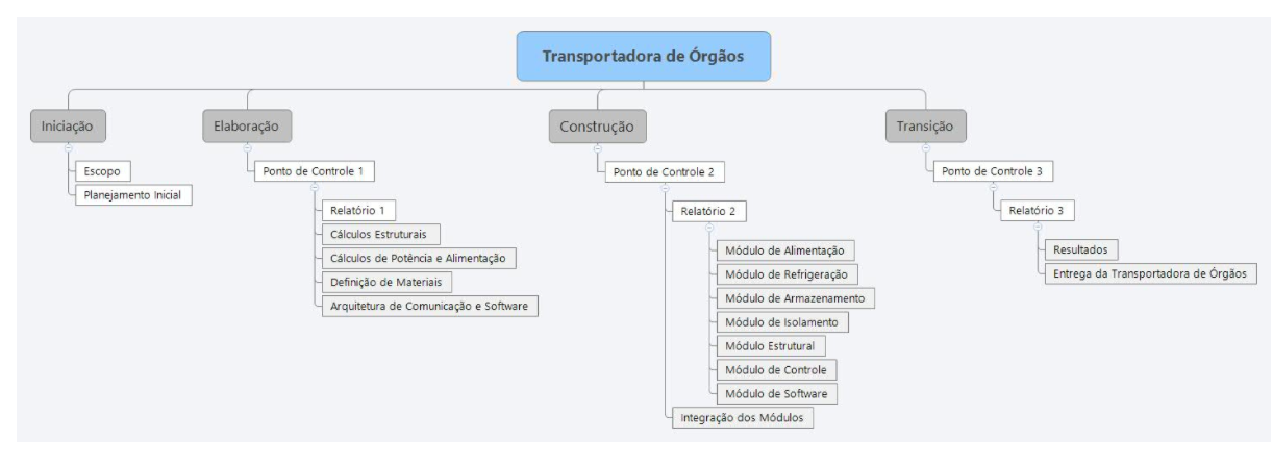
\includegraphics[width=16cm]{figuras/eap.eps}
	\caption{EAP - estrutura analítica do projeto} \label{eap}
\end{figure}

\subsection{Cronograma}

Abaixo segue o cronograma proposto para elaboração do projeto, dividido pelas fases de iniciação, elaboração, construção e transição, seus respectivos marcos e datas limites.

\begin{figure}[H]
	\centering
	\includegraphics[width=16cm]{figuras/cronograma_1.eps}
	\caption{Cronograma do projeto} \label{cronograma_1}
\end{figure}

\begin{figure}[H]
	\centering
	\includegraphics[width=16cm]{figuras/cronograma_2.eps}
	\caption{Cronograma do projeto} \label{cronograma_2}
\end{figure}




